\chapter{Introdução}
\label{ch:introducao}

O transporte de cargas no Brasil depende fortemente das rodovias. O caminhão oferece capilaridade e permite o atendimento porta a porta. Em viagens longas, porém, essa escolha também concentra consumo de diesel, custo operacional e emissões.

A cabotagem é a navegação entre portos do mesmo país. Ela pode substituir parte do percurso rodoviário quando a origem e o destino podem ser ligados por três etapas: acesso rodoviário ao porto, navegação costeira e acesso rodoviário ao destino final \cite{icct2022}. Portanto, a cabotagem não elimina necessariamente o caminhão. Ela muda a função do transporte rodoviário dentro da cadeia.

Um exemplo ajuda a visualizar o problema. Para transportar uma remessa de São Paulo a Manaus, a alternativa rodoviária direta liga as duas cidades por estrada. Uma alternativa multimodal pode levar a carga por rodovia até Santos, transportá-la por navio até Manaus e completar por rodovia o acesso ao destino. A comparação correta deve incluir todas essas etapas. Comparar apenas o navio com o caminhão produziria uma fronteira incompleta.

Neste relatório, o acesso inicial ao porto é chamado de \emph{pre-carriage}. O acesso final, entre o porto de destino e o destino da carga, é chamado de \emph{on-carriage}. A cadeia também pode conter operações portuárias e \emph{hoteling}, isto é, a permanência do navio no porto com sistemas de bordo em funcionamento. A conclusão depende das distâncias de cada trecho, dos portos escolhidos, das fontes dessas distâncias, da carga, do consumo, da alocação e da fronteira metodológica \cite{shortsea2019,modalshiftreview2020}.

\begin{figure}[htbp]
\centering
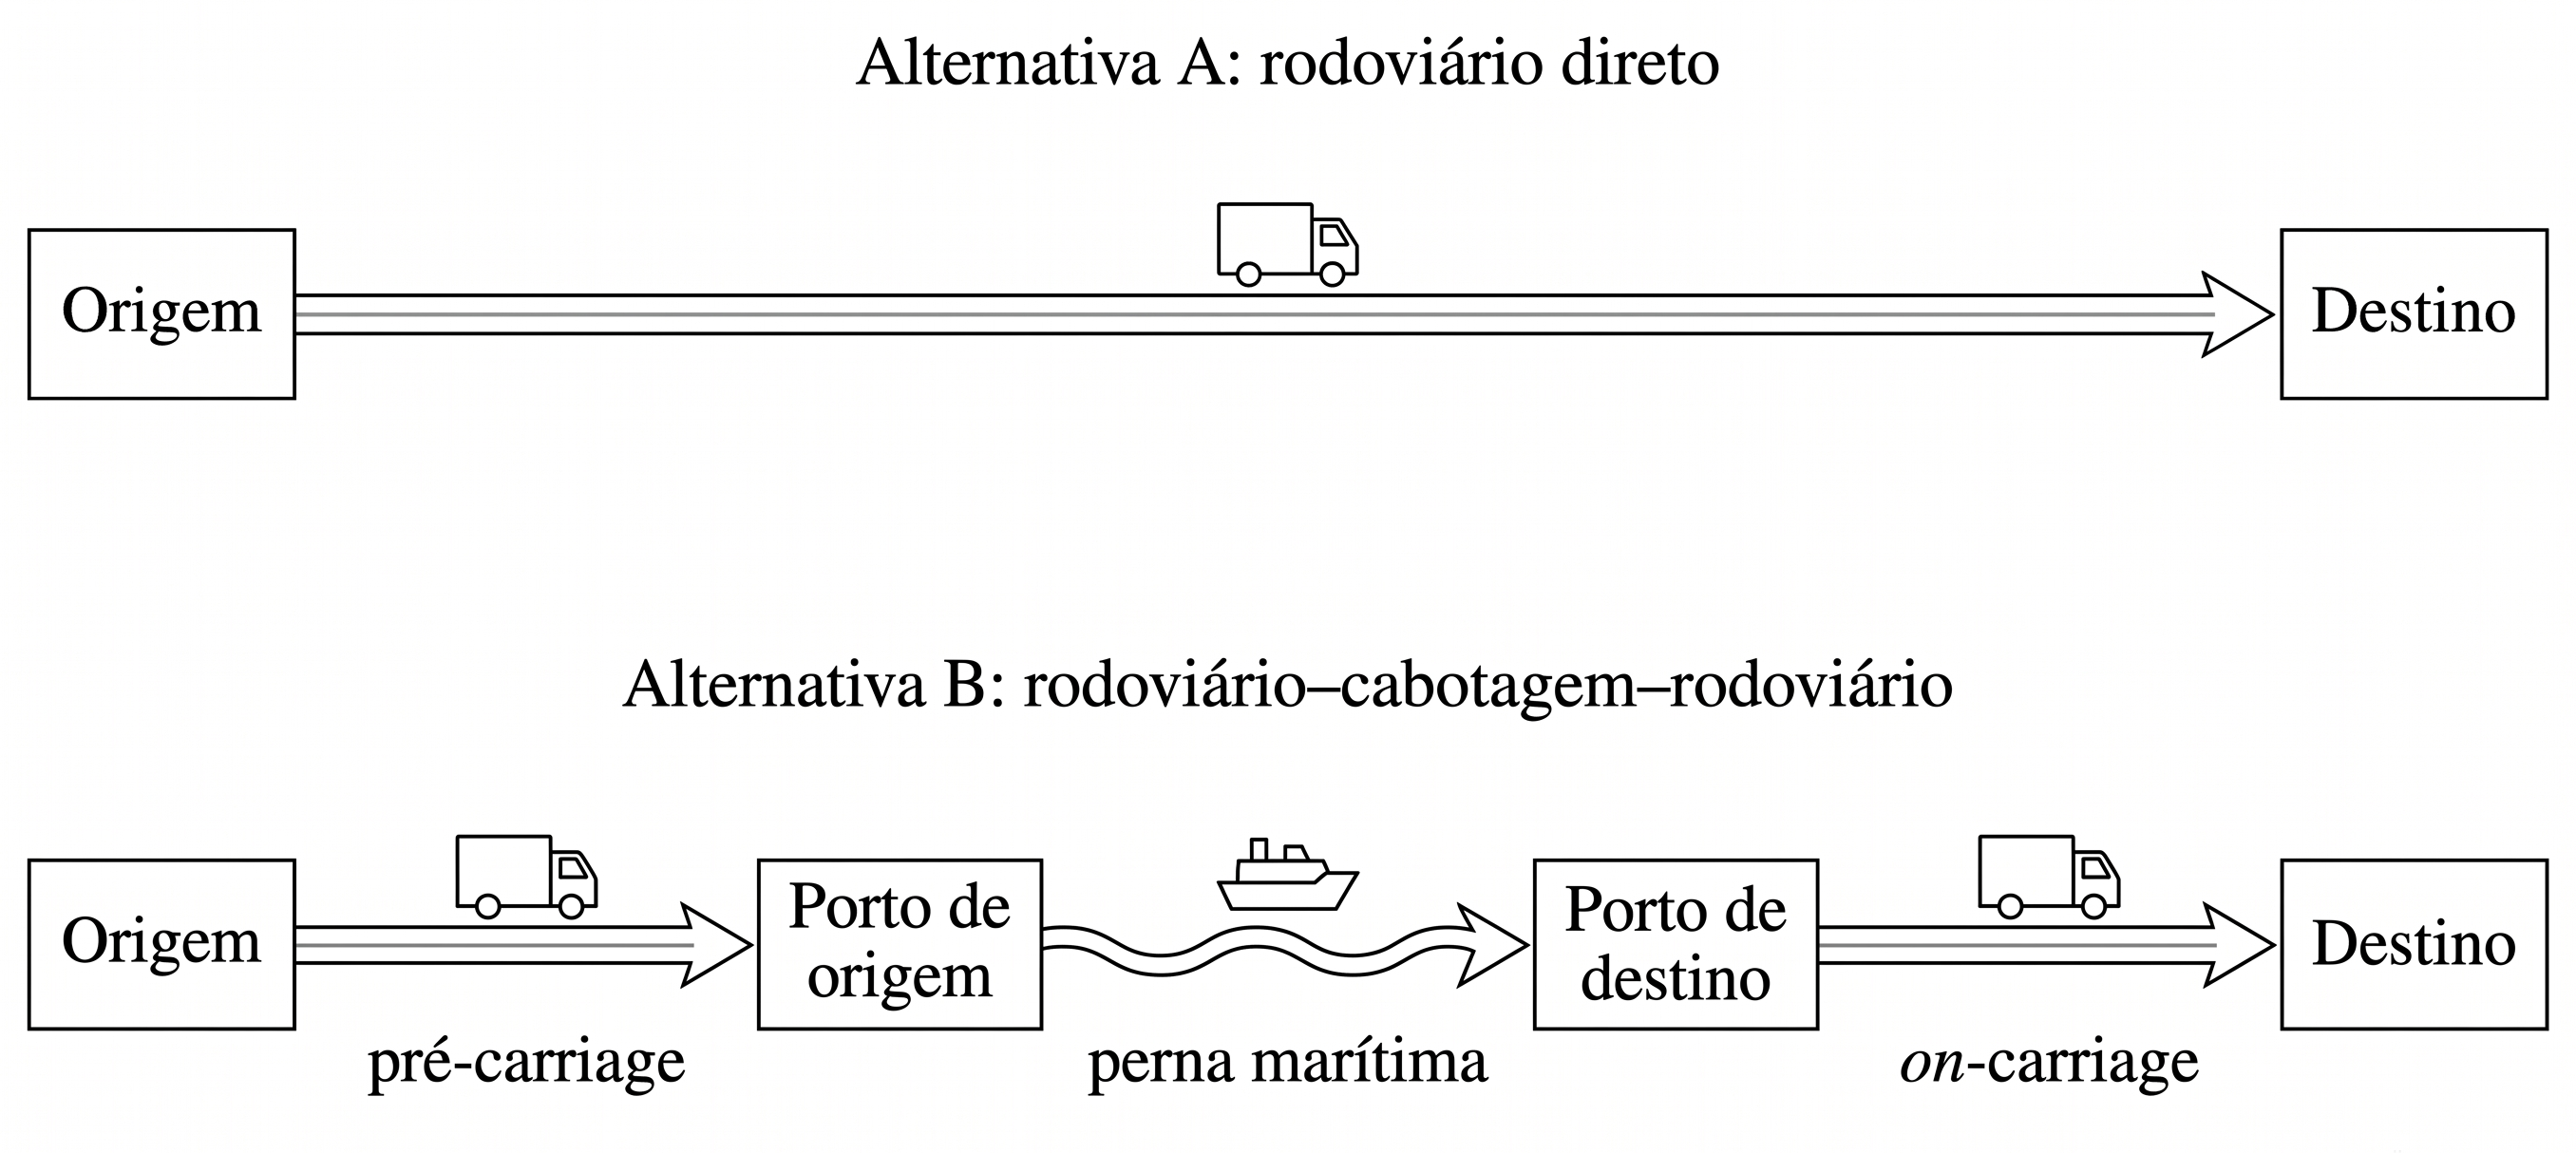
\includegraphics[width=0.95\textwidth]{images/figura_1_1.png}
\caption{Comparação conceitual entre a alternativa rodoviária direta e a cadeia multimodal rodoviária--cabotagem--rodoviária, avaliadas sob a mesma unidade funcional e fronteira porta a porta.}
\label{fig:comparacao-porta-a-porta}
\end{figure}

A Figura~\ref{fig:comparacao-porta-a-porta} resume as duas alternativas. Em ambas, a entrada principal é a mesma remessa, com a mesma origem e o mesmo destino. O processamento muda conforme a cadeia escolhida. A saída reúne distância, consumo, custo modelado e emissões operacionais para cada alternativa.

Decisões logísticas reais também envolvem frequência de serviço, disponibilidade de navios, terminais, tempo de trânsito, confiabilidade, escala, custos comerciais e estrutura de rede \cite{competitiveness2024,modalshiftreview2020}. O escopo deste trabalho é mais específico. Ele constrói uma comparação computacional e rastreável entre a rota rodoviária direta e a cadeia rodoviária--cabotagem--rodoviária. A ferramenta não confirma contratação, frequência ou disponibilidade comercial.

A contribuição central é o \CabotageLens{}. Trata-se de um framework computacional e de um protótipo auditável para comparação acadêmica de alternativas de transporte. Para cada cenário, a ferramenta organiza três grupos de informação:

\begin{itemize}
  \item \textbf{Entradas:} origem, destino, massa da carga, portos e parâmetros técnicos.
  \item \textbf{Processamento:} resolução das rotas, construção das pernas logísticas e cálculo de combustível, custo modelado e emissões.
  \item \textbf{Saídas:} resultados por perna, totais das duas alternativas, fontes utilizadas e avisos de qualidade.
\end{itemize}

Na perna marítima, o método combina as tabelas de Carga e Atracação da ANTAQ com os indicadores de eficiência do EU MRV. Primeiro, o sistema ordena as escalas de cada viagem. Depois, identifica todos os casos em que o porto de origem aparece antes do porto de destino. Uma viagem direta e outra com escalas intermediárias são válidas, desde que respeitem essa ordem.

Em seguida, a carga a bordo é reconstruída em cada subtrecho. O trabalho de transporte da viagem é calculado com a carga e a distância de cada trecho. A intensidade do navio é procurada pelo número IMO no EU MRV. Quando não há correspondência, usa-se uma estatística robusta da classe ou do tipo de embarcação. A fonte escolhida acompanha o resultado. Por fim, a intensidade representativa do par de portos é obtida pela mediana das intensidades das viagens elegíveis, ponderada pelo trabalho de transporte.

O protótipo prioriza recursos computacionais acessíveis. Quando aplicável, utiliza bibliotecas de código aberto e serviços públicos, gratuitos ou com camada gratuita. Essa escolha facilita a reprodução acadêmica e a inspeção dos cálculos. Ela não representa, entretanto, uma garantia de que provedores externos permanecerão gratuitos ou disponíveis.

\methodnote{\textbf{Como ler a fronteira do trabalho.} A saída ambiental representa emissões operacionais \ttw{} de \cooe{}. A saída econômica é um proxy de custo operacional modelado. Ela não é uma cotação de frete.}

Operações portuárias e \emph{hoteling} seguem a fronteira do indicador marítimo utilizado. As operações portuárias permanecem explícitas quando há proveniência documentada. Quando se aplica a intensidade marítima por trabalho de transporte do MRV, o consumo anual reportado do navio é tratado como abrangente para essa finalidade. Nesse caso, o \emph{hoteling} não é somado separadamente, evitando dupla contagem. Se um dado não estiver disponível, o sistema o identifica como indisponível; ele não o transforma em zero.

Assim, o resultado do \CabotageLens{} deve ser lido junto com suas entradas, fontes e limites. A ferramenta mostra quando a alternativa multimodal é promissora dentro da fronteira avaliada. Também mostra quais lacunas impedem uma conclusão mais forte. Essa rastreabilidade é parte do método, e não apenas uma informação adicional.
